\section{Supplementary evidence and robustness}
\label{app:inherited-robustness}

All exercises in this appendix use the same historical sample on which the state was assessed. They measure sensitivity and economic breadth; they do not create a frozen out-of-sample test.

\subsection{Distribution and episode influence}

Removing each portfolio's full-sample bottom-decile months leaves negative carry spot and total state effects. Because the deletion conditions on the realized outcome, it diagnoses tail concentration rather than estimating a preferred conditional mean.

% SOURCE: AI JMP.pdf pp. 39--41, Table 4 and surrounding text.
\begin{table}[H]
\centering
\caption{State effects after removing bottom-decile months}\label{tab:inherited-excrash}
\small
\begin{tabular}{lrrr}
\toprule
Portfolio component & Remaining signal months & Difference (\%/yr) & Episode wild $p$ \\
\midrule
Carry spot       & 77 & -7.24 & 0.006 \\
Carry total      & 77 & -5.50 & 0.024 \\
High-beta spot   & 77 & -3.72 & 0.084 \\
High-beta total  & 78 & -3.68 & 0.060 \\
\bottomrule
\end{tabular}

\vspace{0.35em}
\begin{minipage}{0.94\textwidth}
\footnotesize\emph{Notes:} Each regression drops that return series' full-sample bottom-decile months from both states. The exercise asks whether a few crash observations mechanically generate the conditional-mean result; it does not address selection among alternative signal definitions. Wild-bootstrap $p$-values cluster by IYC episode.
\end{minipage}
\end{table}


The median and every reported lower quantile also move left. For carry spot returns, the monthly median changes from 0.35 percent outside the state to $-0.76$ percent inside, the 25th percentile from $-0.93$ to $-1.98$, and the 10th percentile from $-2.35$ to $-3.94$. This evidence is more informative about a broad distributional shift than the fact that all five worst months occur under the lagged state.

The beta-sorted portfolio exhibits a different distributional pattern. Its bottom-decile frequency is 16.3 percent in active months and 8.5 percent outside them ($p=0.046$); at a fixed $-4$-percent monthly cutoff, the corresponding rates are 9.8 and 4.6 percent ($p=0.033$). Annualized volatility is nearly unchanged, 7.94 versus 7.75 percent, with a variance ratio of 1.05 ($p=0.80$), and reported loss severity conditional on crossing the tail cutoff is similar across states. These outcome-defined diagnostics describe a higher realized tail frequency, not an identified change in disaster probability.

Leave-one-episode-out carry estimates remain within roughly one-third of the full-sample coefficient. The high-beta effect remains statistically detectable under every one-episode deletion, with a largest reported bootstrap $p$-value of 0.006. These checks reduce dependence on a single episode but do not overcome the limited number of episodes.

\subsection{Calendar stability}

The carry-spot coefficient is negative in both calendar halves. The high-beta result is less stable and is concentrated after 2005. The split is descriptive because the rule was not frozen on the first half before evaluation on the second.

% SOURCE: AI JMP.pdf p. 86, Table E.1. Transcribed from PDF; not regenerated.
\begin{table}[H]
\centering
\caption{The headline estimates in two halves of the sample}\label{tab:inherited-halves}
\small
\begin{tabular}{lrrrrrr}
\toprule
& \multicolumn{3}{c}{1988:01--2004:12} & \multicolumn{3}{c}{2005:01--2026:02} \\
\cmidrule(lr){2-4}\cmidrule(lr){5-7}
Series & $b$ & $t_{episode}$ & wild $p$ & $b$ & $t_{episode}$ & wild $p$ \\
\midrule
Carry spot       & -11.41 & -2.54 & 0.037 & -15.85 & -1.99 & 0.010 \\
Carry total      & -10.20 & -2.04 & 0.052 & -14.76 & -1.84 & 0.047 \\
High-beta spot   &  -4.01 & -1.12 & 0.287 & -11.91 & -4.07 & 0.010 \\
High-beta total  &  -3.03 & -0.80 & 0.448 & -11.54 & -3.85 & 0.011 \\
\midrule
Months           & \multicolumn{3}{c}{204} & \multicolumn{3}{c}{254} \\
Signal months    & \multicolumn{3}{c}{54}  & \multicolumn{3}{c}{38} \\
Episodes         & \multicolumn{3}{c}{7}   & \multicolumn{3}{c}{8} \\
\bottomrule
\end{tabular}

\vspace{0.35em}
\begin{minipage}{0.94\textwidth}
\footnotesize\emph{Notes:} Each column reports the state regression $y_t=a+b\,\mathbf{1}\{\mathrm{IYC}\}_{t-1}+e_t$ estimated separately by calendar half. Coefficients are annualized percentage points; $t_{episode}$ clusters by IYC episode, and wild-bootstrap $p$-values use $B=9{,}999$. This is a stability check, not a frozen out-of-sample test.
\end{minipage}
\end{table}


\subsection{State-definition sensitivity}

The reported grids vary breadth, release confirmation, and the short maturity. Separate exactly-one and exactly-two indicator regressions have coefficients with opposite signs; they are not a direct contrast because each indicator is compared with a different complement. At-least-three and at-least-four rules have fewer active months and later coverage. Releasing after one steepening month is noisier; requiring three retains the state longer. Rebuilding the state with a 10Y--3M rather than 10Y--2Y slope preserves the broad adverse ordering but changes episode timing.

The raw current-inversion state is active in 165 months, compared with 92 for the live state. Relative to the raw count, the live state improves tail concentration rather than absolute capture at every cutoff. The raw count contains 9 of the 23 worst-5-percent months and 19 of the 46 worst-10-percent months, versus 8 and 15 for the live state. Because the raw count is active in 36 percent of the sample rather than 20 percent, its concentration ratios are lower---1.09 versus 1.73 at the 5-percent cutoff and 1.15 versus 1.62 at the 10-percent cutoff. Only in the extreme five-month tail does the live state dominate absolute capture, 5 of 5 versus 2 of 5. The latch can retain losses that arrive after curves begin to re-steepen, but its extreme-tail concentration is partly mechanical because the historical crash chronology helped motivate persistence.

Breadth above two mainly measures episode maturity rather than a monotone risk dose. Months with at least three live curves have median episode age six months, compared with three months for exactly-two months, and eleven of fifteen episodes begin at exactly two. Conditional on the baseline state, a three-or-more indicator adds no reported information with or without episode-age controls ($p\geq0.27$). The exact-two contrast is therefore an entry/configuration result, not evidence that each additional inversion raises loss risk.

A reciprocal-age version of the current-inversion count separates two timing margins. It has a high-beta spot coefficient of $-14.87$ ($p=0.001$), larger than the baseline live state's $-7.53$, but a smaller carry coefficient of $-10.43$ ($p=0.040$) than the baseline's $-12.85$. Under the full control set, the age-weighted high-beta coefficient remains $-13.82$ ($p=0.008$), whereas its carry coefficient attenuates to $-7.55$ ($p=0.084$). These in-sample comparisons suggest that exposure repricing is concentrated near fresh information, while the path-dependent release rule is more important for carry losses that continue into re-steepening.

% SOURCE: AI JMP.pdf pp. 79 and 94, Tables C.3 and K.1. Transcribed, not regenerated.
\begin{table}[H]
\centering
\caption{Measurement perturbations and exposure ordering}
\label{tab:measurement-perturbations}
\small
\begin{tabular}{lrrrr}
\toprule
State construction & Carry spot & Wild $p$ & High-beta spot & Wild $p$ \\
\midrule
10Y--2Y baseline & $-12.85$ & 0.001 & $-7.53$ & 0.010 \\
10Y--3M slope & $-4.68$ & 0.146 & $-5.25$ & 0.011 \\
U.S.-term-premium-adjusted 10Y--2Y & $-5.42$ & 0.107 & $-6.17$ & 0.004 \\
\bottomrule
\end{tabular}

\begin{minipage}{0.94\textwidth}
\footnotesize\emph{Notes:} Coefficients are annualized percentage-point active-state differences. The 10Y--3M row rebuilds every curve state using a different short maturity. The term-premium row removes each national slope's fitted exposure to the U.S. ACM 10Y-minus-2Y slope premium before rebuilding the state. Both perturbations attenuate carry while retaining the beta-sorted exposure result.
\end{minipage}
\end{table}


\begin{table}[H]
\centering
\caption{State-definition multiverse: reported and untested dimensions}
\label{tab:multiverse}
\small
\begin{tabularx}{\textwidth}{>{\raggedright\arraybackslash}p{3.1cm} >{\raggedright\arraybackslash}X >{\raggedright\arraybackslash}X}
\toprule
Dimension & Reported neighborhood & Remaining uncertainty \\
\midrule
Breadth & At least 1--4; exactly 1--2 & Frequency-matched and country-combination rules \\
Release & One-, two-, and three-month confirmation & Other persistence and duration-matched placebo rules \\
Tenor & 10Y--2Y baseline; 10Y--3M check & Other maturities and inversion cutoffs \\
Freshness & Fresh crossing versus current inversion & Alternative age decay and entry delay \\
Geography & Non-U.S. G10 baseline; U.S.-inclusion checks & Other developed-market sets and country combinations \\
Portfolio & Three-by-three carry and beta sorts & Other leg sizes, volatility scaling, feasible forwards \\
Timing & Month-end recursion and one extra lag & Vendor timestamps, asynchronous closes, vintage data \\
\bottomrule
\end{tabularx}
\end{table}

\subsection{Bilateral cluster and own-curve specifications}

The full country-level horse race is reported below. The cluster includes the focal country's curve in every row. These regressions ask whether the configuration remains informative after controlling for the currency's own state and slope variables; they do not show that other countries' curves alone predict the focal currency.

% SOURCE: AI JMP.pdf p. 49, Table 8. Exact native transcription; not regenerated.
% IMPORTANT: The cluster includes the focal country's curve. This is not a leave-one-country-out design.
\begin{table}[H]
\centering
\caption{Bilateral cluster and own-curve specifications}
\label{tab:v03-bilateral-own-curve}
\scriptsize
\setlength{\tabcolsep}{3pt}
\begin{tabular}{lrrrr}
\toprule
Currency & Own-state months & Own state alone & Cluster alone \\
& & $b\;(t_{NW})\;[p]$ & $b\;(t_{NW})\;[p]$ \\
\midrule
AU & 47 & $-8.76\;(-1.65)\;[0.044]$ & $-13.21\;(-1.83)\;[0.015]$ \\
CA & 40 & $+0.71\;(+0.19)\;[0.858]$ & $-4.61\;(-1.33)\;[0.203]$ \\
CH & 12 & $-20.12\;(-1.91)\;[0.303]$ & $-0.89\;(-0.16)\;[0.867]$ \\
EU & 25 & $+5.26\;(+0.62)\;[0.589]$ & $-1.19\;(-0.20)\;[0.831]$ \\
GB & 59 & $-3.84\;(-0.59)\;[0.585]$ & $-3.00\;(-0.63)\;[0.542]$ \\
JP & 22 & $+4.58\;(+1.03)\;[0.298]$ & $+2.35\;(+0.58)\;[0.565]$ \\
NO & 82 & $+4.53\;(+0.84)\;[0.415]$ & $-3.96\;(-0.71)\;[0.520]$ \\
NZ & 48 & $-11.42\;(-1.33)\;[0.282]$ & $-13.28\;(-1.99)\;[0.011]$ \\
SE & 13 & $-13.05\;(-1.02)\;[0.497]$ & $-4.94\;(-0.76)\;[0.416]$ \\
Pooled (currency FE) & --- & --- & $-4.74\;(-2.34)\;[---]$ \\
\bottomrule
\end{tabular}

\vspace{0.7em}
\begin{tabular}{lrrrl}
\toprule
Currency & Cluster, with own state & Own state, with cluster & Full-spec. cluster & Own-curve joint Wald $p$ \\
& $b\;(t_{NW})\;[p]$ & $b\;(t_{NW})\;[p]$ & $b\;(t_{NW})\;[p]$ & \\
\midrule
AU & $-14.18\;(-1.38)\;[0.133]$ & $+2.19\;(+0.23)\;[0.859]$ & $-12.92\;(-1.31)\;[0.262]$ & 0.408 \\
CA & $-6.01\;(-1.45)\;[0.207]$ & $+4.50\;(+1.04)\;[0.356]$ & $-5.55\;(-1.46)\;[0.282]$ & 0.801 \\
CH & $+1.28\;(+0.21)\;[0.848]$ & $-20.95\;(-1.81)\;[0.272]$ & $+1.15\;(+0.18)\;[0.875]$ & 0.115 \\
EU & $-3.40\;(-0.51)\;[0.584]$ & $+8.13\;(+0.80)\;[0.552]$ & $-4.00\;(-0.61)\;[0.560]$ & 0.488 \\
GB & $-2.00\;(-0.45)\;[0.622]$ & $-2.82\;(-0.44)\;[0.668]$ & $-0.44\;(-0.10)\;[0.928]$ & 0.486 \\
JP & $+1.68\;(+0.38)\;[0.733]$ & $+3.41\;(+0.71)\;[0.413]$ & $+6.37\;(+1.32)\;[0.251]$ & 0.006 \\
NO & $-6.85\;(-1.15)\;[0.289]$ & $+7.43\;(+1.42)\;[0.221]$ & $-8.17\;(-1.23)\;[0.281]$ & 0.233 \\
NZ & $-12.00\;(-2.06)\;[0.011]$ & $-3.22\;(-0.41)\;[0.748]$ & $-8.56\;(-1.26)\;[0.220]$ & 0.373 \\
SE & $-3.73\;(-0.61)\;[0.526]$ & $-10.58\;(-0.92)\;[0.540]$ & $-2.99\;(-0.48)\;[0.662]$ & 0.150 \\
Pooled (currency FE) & $-4.74\;(-2.34)\;[---]$ & $-0.01\;(-0.01)\;[---]$ & --- & --- \\
\bottomrule
\end{tabular}

\begin{minipage}{0.97\textwidth}
\footnotesize\emph{Notes:} Spot returns against the U.S. dollar, 1988:01--2026:02. Each compact cell reports the annualized coefficient, Newey--West (12) $t$-statistic in parentheses, and wild episode-bootstrap $p$-value in brackets. The full specification adds the currency's own 10Y--2Y slope, its one-month change, its slope relative to the U.S. curve, and the average G10 slope and change. The final column is the Newey--West Wald $p$-value for the joint null on that currency's own state, relative slope, and relative level conditional on the cluster. The pooled row reports currency fixed effects and no bootstrap inference. The cluster used in every row includes the focal country's curve. This table conditions on own-curve information; it is not a leave-one-country-out signal.
\end{minipage}
\end{table}


\subsection{Exposure breadth and composition}

The carry and beta portfolios have persistent cores rather than changing membership only when the state turns on. New Zealand occupies the high-rate leg in 85 percent of all months and 91 percent of state months; Australia in 71 and 73 percent. Japan and Switzerland remain the principal funding currencies. There is also rotation around the core: Norway's carry-long share falls from 62 to 34 percent in state months, while the pound's rises from 43 to 70 percent. The return result is therefore not created solely by state-month resorting, but portfolio composition is not fixed.

% SOURCE: AI JMP.pdf p. 91, Table H.1. Exact full-sample and active-state entries for all nine currencies.
\begin{table}[H]
\centering
\caption{Complete portfolio composition in the full sample and active state}
\label{tab:v03-portfolio-composition-full}
\footnotesize
\begin{tabular}{lrrrr}
\toprule
& \multicolumn{2}{c}{Long share} & \multicolumn{2}{c}{Funding share} \\
\cmidrule(lr){2-3}\cmidrule(lr){4-5}
Currency & Full & State & Full & State \\
\midrule
\multicolumn{5}{l}{\emph{Panel A: carry portfolio}} \\
New Zealand & 85 & 91 & 2 & 1 \\
Australia & 71 & 73 & 4 & 0 \\
Norway & 62 & 34 & 3 & 5 \\
United Kingdom & 43 & 70 & 4 & 0 \\
Canada & 20 & 21 & 23 & 14 \\
Sweden & 15 & 12 & 33 & 36 \\
Euro area & 4 & 0 & 51 & 47 \\
Japan & 0 & 0 & 83 & 97 \\
Switzerland & 0 & 0 & 96 & 100 \\
\addlinespace
\multicolumn{5}{l}{\emph{Panel B: equity-beta portfolio}} \\
Canada & 100 & 100 & 0 & 0 \\
Australia & 97 & 92 & 0 & 0 \\
New Zealand & 77 & 76 & 0 & 0 \\
Norway & 26 & 32 & 0 & 0 \\
Euro area & 0 & 0 & 46 & 45 \\
United Kingdom & 0 & 0 & 52 & 47 \\
Sweden & 0 & 0 & 34 & 59 \\
Japan & 0 & 0 & 73 & 65 \\
Switzerland & 0 & 0 & 95 & 85 \\
\bottomrule
\end{tabular}

\begin{minipage}{0.82\textwidth}
\footnotesize\emph{Notes:} Entries are percentages of months in which each currency appears in the indicated three-currency leg. Full denotes all 458 portfolio months; State denotes the 92 active-state months. Column sums can differ slightly from 300 because the displayed shares are rounded to integer percentages.
\end{minipage}
\end{table}


The seven floating emerging-market currencies are not used to construct the G10 state. All seven bilateral state coefficients are negative; only the rand is individually detected at conventional levels ($-14.68$, $p=0.015$), while the rupee is marginal ($-7.98$, $p=0.061$) and the other five estimates are imprecise. Pooled spot and total effects are $-14.37$ and $-13.35$ percentage points per year, with episode-bootstrap $p$-values of 0.104 and 0.079. In the same EM panel, source-reported pooled spot coefficients are $-4.54$ for the raw current count and $-3.92$ for its six-month age filter. This ordering favors the live construction in sample, but all three designs use the same global dates and the live estimate itself is imprecise at the episode level.

The common-sample comparison separates international spot repricing from compensation.

% SOURCE: AI JMP.pdf pp. 53--55, Tables 11--12. Transcribed, not regenerated.
\begin{table}[H]
\centering
\caption{Spot repricing and compensation across currency universes, 1996--2026}
\label{tab:g10-em-compensation}
\small
\begin{tabular}{llrrrr}
\toprule
Universe & Return leg & Inactive mean & Active mean & State difference & Episode wild $p$ \\
\midrule
G10 & Spot & 2.96 & $-12.79$ & $-15.75$ & $<0.001$ \\
G10 & Total & 6.22 & $-8.67$ & $-14.89$ & 0.003 \\
G10+EM & Spot & 0.46 & $-12.51$ & $-12.97$ & 0.176 \\
G10+EM & Total & 11.68 & 2.51 & $-9.18$ & 0.235 \\
\bottomrule
\end{tabular}

\begin{minipage}{0.94\textwidth}
\footnotesize\emph{Notes:} Annualized percentages over the common 1996:01--2026:02 sample. The G10+EM universe adds seven floating emerging-market currencies and applies the same three-by-three rate sort. Active-state income implied by total minus spot is approximately 4.12 percent for G10 and 15.02 percent for G10+EM. The nearly equal spot means but different total means show how predetermined carry income changes the payoff from similar currency repricing.
\end{minipage}
\end{table}


The combined sort is economically concentrated. Emerging-market currencies occupy 99 percent of carry-long slots and 93 percent of high-beta-long slots; the Brazilian real alone enters the carry-long leg in 93 percent of months. The comparison is therefore close to a persistent emerging-market exposure against the yen--franc--euro funding bloc, not a broadly rotating sixteen-currency portfolio.

Baseline exposure tests use expanding S\&P 500 betas. An oil-beta sort adds little independent variation because its return is largely spanned by the carry and equity-beta portfolios.

\subsection{Conditional UIP and macro timing}

Appendix~\ref{app:theory} gives the conditional Fama specification. The pooled slope is 0.50 outside the state and $-1.33$ inside, but the state interaction has episode-bootstrap $p=0.340$. The point estimate is consistent with high-rate currencies depreciating during the state, while the interaction remains imprecise at the episode level.

\begin{figure}[p]
    \centering
    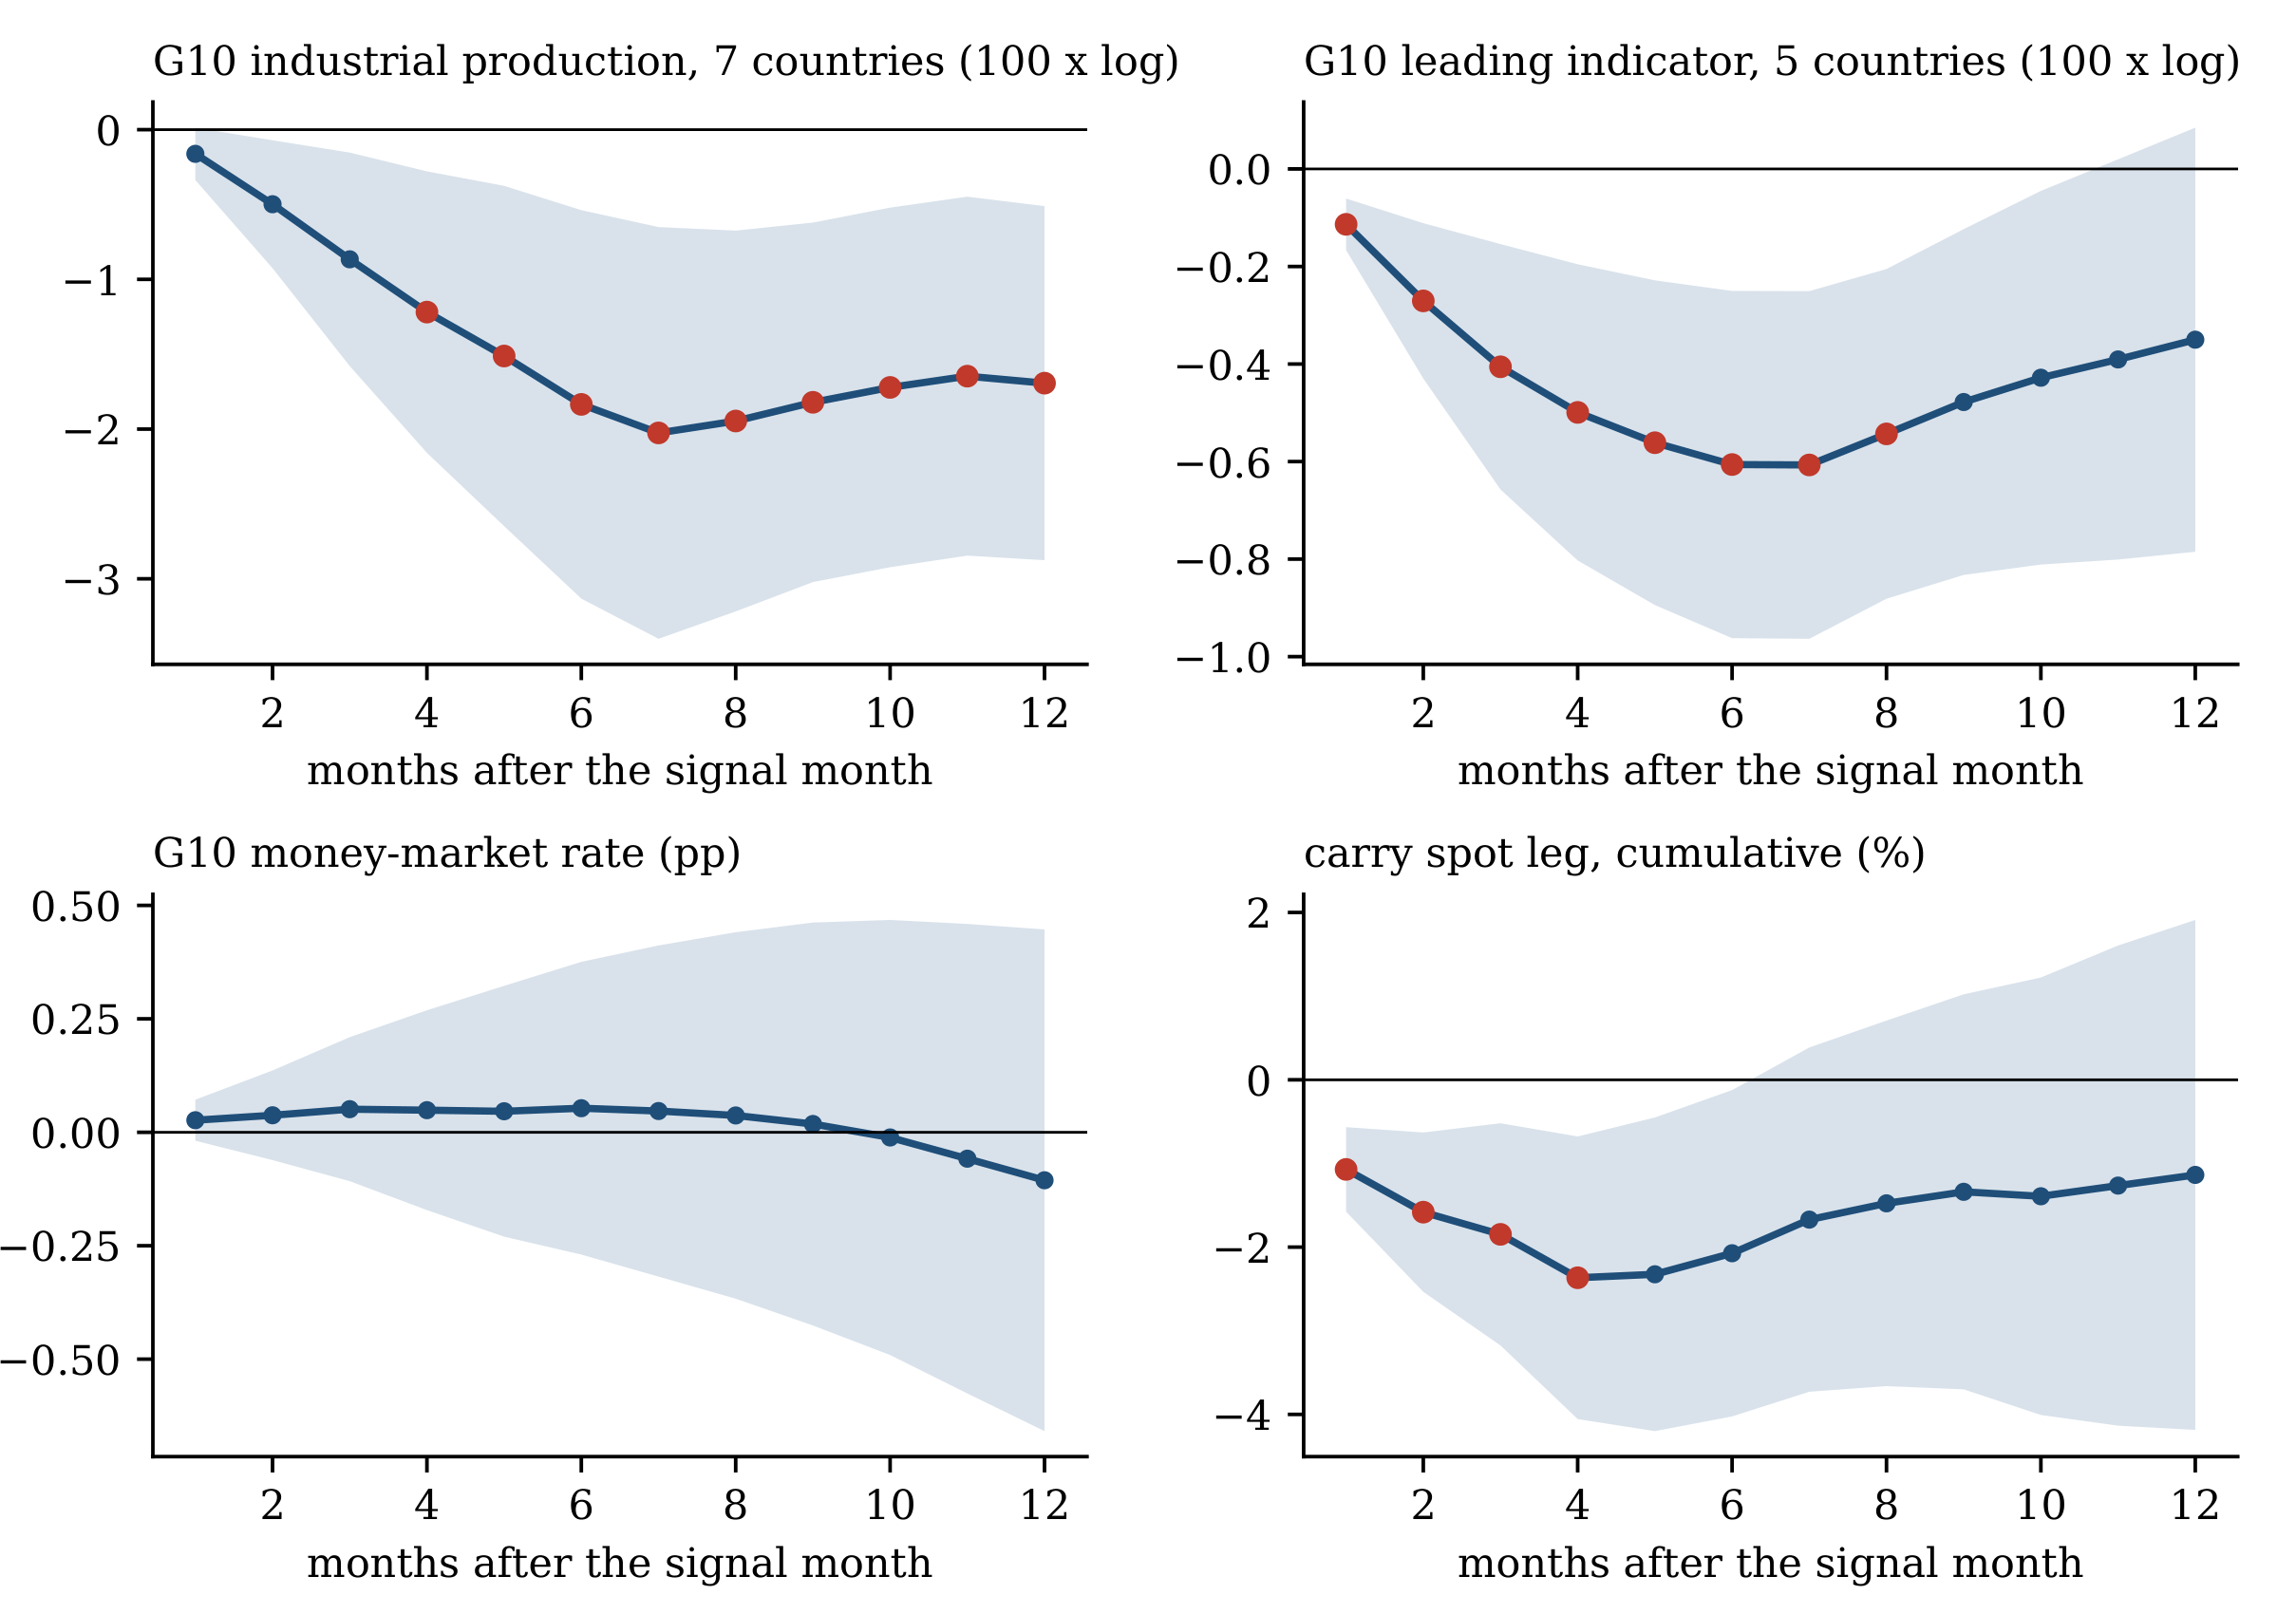
\includegraphics[width=\textwidth]{assets/original/figure_06_main.png}
    \caption{Outcomes following a synchronized-inversion state. The panels show local projections of cumulative changes in G10 industrial production, the OECD composite leading indicator, the average G10 money-market rate, and the carry spot leg. Bands are 90-percent Newey--West intervals; markers denote episode-bootstrap $p<0.10$. Overlapping horizons and persistent states make these supporting temporal associations rather than causal responses.}
    \label{fig:inherited_local_projections}
\end{figure}

The carry-spot response is front-loaded. In the baseline projection it falls about 1.1 percent in the first month ($p<0.01$) and 2.4 percent cumulatively by month four ($p=0.06$). Onset-only and lag-controlled designs reach roughly $-3.7$ to $-4.2$ percent around months four through six, followed by a partial rebound. Because horizons overlap and the state is persistent, these are descriptive timing associations rather than causal impulse responses.

The leading indicator declines by about 0.6 percent over six months, with similar magnitudes around episode onsets and under lag controls. Industrial production declines about 1.8 percent at six months in the baseline projection but becomes imprecise with the fullest controls. The average G10 money-market rate is approximately flat for the following year across the baseline, onset, and controlled projections. The leading-indicator response is persistent across these specifications; the industrial-production response and a uniform coordinated-easing path are not.

\subsection{Benchmarks, controls, and term premia}

The U.S. inversion, average G10 slope, and its change do not span the synchronized state. Lagged NFCI and VIX controls also leave the carry coefficient near its baseline magnitude. Contemporaneous dollar and FX-volatility controls show that the realized loss is not simply the average dollar move or the measured volatility innovation, but they are not predictive controls.

Substituting G10 implied-volatility innovations preserves carry coefficients but weakens high-beta inference: high-beta point estimates remain near $-7.5$ percentage points and have $p$-values around 0.17--0.18. The raw current-inversion count is absorbed by the full NFCI/VIX set, with carry $p\geq0.58$ and high-beta $p\geq0.12$. These adverse cells prevent the control evidence from being read as uniform across volatility measures or state constructions.

The term-premium adjustment is asymmetric. After removing fitted exposure to the U.S. ACM 10Y-minus-2Y term-premium slope, 83 percent of national inversions remain. The rebuilt state still contains all five worst carry months, but it expands from 92 to 125 active months. The high-beta coefficient is $-6.2$ percentage points with $p=0.004$, while the carry coefficient is about $-5.4$ with $p=0.11$. The smaller carry estimate reflects a changed classifier---and possible dilution from the additional months---as well as removal of fitted exposure to the U.S. premium. The exercise does not identify what share of the baseline association is attributable to a common term-premium component. Comparable foreign-country decompositions are unavailable.

\subsection{Interpretive boundary}

The conditional return gap, distributional shift, and exposure ordering are statistically detectable in the reported specifications. The conditional-UIP interaction and industrial-production response are imprecise; emerging-market breadth and the downcurve split are exploratory. Feasible forward returns, complete data-vintage auditing, a comprehensive state multiverse, and a frozen future sample remain untested.
